\section{ST-structures and HDAs}
\label{sec:st-structure-and-hda}

    For ST-structures to precisely identify events in higher-dimensional automata we need a way of translating ST-structures into higher-dimensional automata. Johansen in \cite{Johansen16STstruct} provides a way of translating ST-structures into higher-dimensional automata as follows.

    \begin{definition}[$\allST$ to $\allHDA$ \cite{Johansen16STstruct}]
        \label{def:ST-structures-to-HDA}
        We define a mapping $\stintoh : \allST \rightarrow \allHDA$ from ST-structures into $\HDA$s which for an $\ST=(E,ST,l)$ with the events linearly ordered as a list $\evlist{E}$ (that is, each event being indexed by a natural number, as in a sequence) returns the $\HDA$ $\stintoh(\ST)$ which
    
        \begin{itemize}
            \item has cells $\mathcal{Q} = \{q^{(\mathcal{S},\mathcal{T})}\in \mathcal{Q}_{n} \mid (\mathcal{S},\mathcal{T})\in ST \mbox{ and } |\mathcal{S} \setminus \mathcal{T}|=n\}$;
            \item for any two cells $q^{(\mathcal{S},\mathcal{T})}$ and $q^{(S\setminus e,T)}$ add the map entry $s_{i}(q^{(\mathcal{S},\mathcal{T})})=q^{(\mathcal{S} \setminus e,\mathcal{T})}$ where $i$ is the index of the event $e$ in the listing $\evlist{E}\!\!\downarrow_{(\mathcal{S} \setminus \mathcal{T})}$;
            \item for any two cells $q^{(\mathcal{S},\mathcal{T})}$ and $q^{(\mathcal{S},\mathcal{T} \cup e)}$ add the map entry $t_{i}(q^{(\mathcal{S},\mathcal{T})})=q^{(\mathcal{S},\mathcal{T} \cup e)}$ where $i$ is the index of the event $e$ in the listing $\evlist{E}\!\!\downarrow_{(\mathcal{S} \setminus \mathcal{T})}$;
            \item has labelling $l(q^{(\mathcal{T} \cup e,\mathcal{T})})=l(e)$ for any $q^{(\mathcal{T} \cup e,\mathcal{T})}\in \mathcal{Q}_{1}$.
        \end{itemize}

        More precisely, by $\evlist{E}\!\!\downarrow_{(\mathcal{S} \setminus \mathcal{T})}$ we represent the listing of the events in $\mathcal{S} \setminus \mathcal{T}$, namely, a list of dimension $|\mathcal{S} \setminus \mathcal{T}|$ obtained from the original listing $\evlist{E}$ by removing all other events. This new listing has the events of $\mathcal{S} \setminus \mathcal{T}$ in the same original order but with new indexes attached (ranging from $1$ to $|\mathcal{S} \setminus \mathcal{T}|$).
    \end{definition}

    As shown in \cite[Theorem 3.36]{Johansen16STstruct}, the mapping $\stintoh$ associates a rooted, connected, and adjacent-closed ST-structure with $\stintoh(\ST)$, which is a higher-dimensional automaton respecting the precubical identities and is acyclic. The non-degenerate property of higher-dimensional automata is defined by the underlying precubical set. Hence, the property of non-degeneracies is preserved. As shown by Johansen in \cite[Lemma 3.37]{Johansen16STstruct}, the way the events are picked in the definition of the mapping $\stintoh$ do not matter.

    \begin{example}[Strong asymmetric conflict]
        \label{exp:asymmetric-conflict}
        This example is taken from \cite[Example 3.38]{Johansen16STstruct}, but can also be found in \cite[Example 3]{GlabbeekP09configStruct}, and in \cite[page.22]{Pratt03trans_cancel} the asymmetric conflict is considered \emph{strong}. 
    
        \begin{figure}[ht]
            \centering
            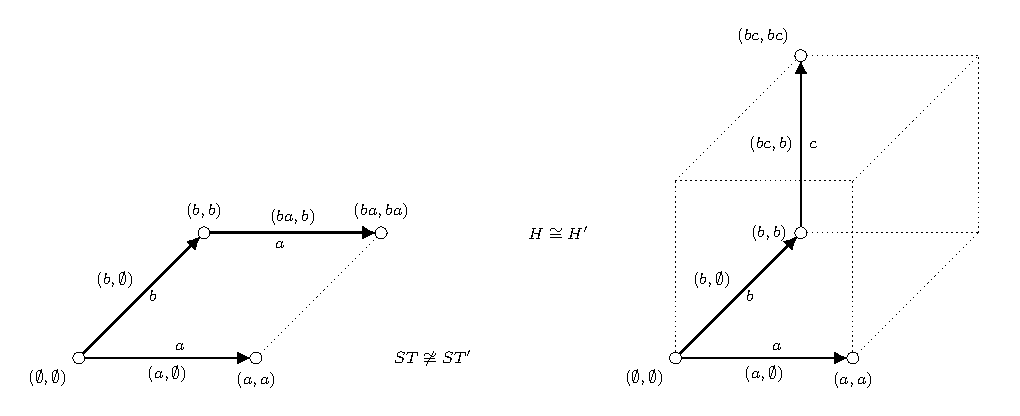
\includegraphics[scale=0.9]{Figures/4.Relationship-with-other-models-of-concurrency/ST-structure-and-HDA/Asymmetric-conflict.pdf}
            \captionof{figure}[Asymmetric conflict]{Example of ST-structures and higher-dimensional automata representing the asymmetric conflict $a + b$. The higher-dimensional automaton (left) is isomorphic to the higher-dimensional automaton (right). On the other hand, we see that the ST-structure (left) is not isomorphic to the ST-structure (right). Since, the ST-structure (left) is on two events and the ST-structure (right) is on three events.}
            \label{fig:asymmetric-conflict-st-hda}
        \end{figure}
    
        The example has no concurrency and involves two events, imposing the only restriction that once event $a$ happens, then event $b$ cannot occur anymore. 
    
        Higher-dimensional automata are not good at identifying the particular events, making the representation of the example as a higher-dimensional automaton challenging. Higher-dimensional automata are state-based models that represent events by actions, where actions are labels for the particular events. These actions may occur multiple times, where events only occur once in an execution. The standard way of identifying events in higher-dimensional is by equivalence classes of transitions, where two transitions are equivalent when they are parallel in the boundary of a filled square, see Figure \ref{fig:HDA-filled-interleaving-square}.
    
        The equivalence classes of transitions for higher-dimensional automata, shown in Figure \ref{fig:asymmetric-conflict-st-hda} (left), would not result in the corresponding 2-event ST-structure, which is what we want. However, would result in the 3-event ST-structure of Figure \ref{fig:asymmetric-conflict-st-hda} (right). The 2-event ST-structure is not isomorphic to the 3-event ST-structure. On the other hand, the two representations of the higher-dimensional automata from Figure \ref{fig:asymmetric-conflict-st-hda} (left and right) are isomorphic.
    \end{example}
    
    In \cite[Proposition 3.39]{Johansen16STstruct}, the mapping $\stintoh$ from Definition~\ref{def:ST-structures-to-HDA} preserves isomorphism. However, it may collapse non-isomorphic ST-structures into isomorphic higher-dimensional automata. Consider the two ST-structures from Figure~\ref{fig:asymmetric-conflict-st-hda} which are not isomorphic since the left one is defined by two events while the right one is defined by three events, whereas the higher-dimensional automata that the mapping $\stintoh$ associates are isomorphic. This means that $\stintoh$ is not an embedding from $\allST$ to $\allHDA$ since it looses information, namely, the events. A natural question to raise is if a mapping from $\allHDA$ to $\allST$ is then an embedding from $\allHDA$ to $\allST$. We will first define a mapping from $\allHDA$ to $\allST$.
    
    \begin{definition}[Events equivalence relation of $\HDA$ \cite{Johansen16STstruct}]
        \label{def:events-equivalence-relation-of-HDA}
        Define a relation $\eventEquivHDAs\ \subseteq \mathcal{Q}_{1}\times \mathcal{Q}_{1}$ on transitions of $\mathcal{H}$ as 
        
        \[
            q_{1}\eventEquivHDAs q_{1}' \quad\text{iff}\quad \exists q_{2}\in
            \mathcal{Q}_{2}:\alpha_{i}(q_{2})=q_{1}\wedge \beta_{i}(q_{2})=q_{1}'
        \]
        for some $i\leq 2$ and $\alpha,\beta\in\{s,t\}$.  Consider the reflexive and transitive closure of the above relation, and denote it the same. This is now an equivalence relation on $\mathcal{Q}_{1}$.
        % Consider an equivalence class $\equivClass{q_{1}}$ to be all
        % $q_{1}'$ equivalent with $q_{1}$.  Such an equivalence class is
        % called \emph{an event}.
    \end{definition}
    

    \begin{definition}[$\allHDA$ to $\allST$ \cite{Johansen16STstruct}]
        \label{def:HDA-to-ST-structure}
         Define a map $\ST:\allHDA \rightarrow \allST$ which builds an ST-structure $\ST(\mathcal{H})$ by associating to each rooted path $\pi\in \mathcal{H}$ an ST-configuration as follows.

        \begin{enumerate}
            \item\label{hintost_1} for the minimal rooted path which ends in $I$ associate $(\emptyset,\emptyset)$;
            \item\label{hintost_2} for any path $\pi$ which ends in a transition $\finishPath{\pi}=q_{1}\in \mathcal{Q}_{1}$ then 
        
            \begin{enumerate}
                \item\label{hintost_21} add the ST-configuration $\hintost(\pi)=\hintost(\pi_{s})\cup(\equivClass{q_{1}},\emptyset)$, where $\pi_{s}$ is a shorter path reaching through an s-map the homotopy class of $\pi$, that is, $\pi_{s}\transition{s}q_{1}\in\homotopyClass{\pi}$;
                \item\label{hintost_22} add the ST-configuration $\hintost(\pi\transition{t}q_{0})=\hintost(\pi)\cup(\emptyset,\equivClass{q_{1}})$;
            \end{enumerate}

            \item\label{hintost_3} for any path $\pi$ which ends in a higher cell $\finishPath{\pi}=q_{n}\in \mathcal{Q}_{n}$, with $n\geq 2$, then add the ST-configuration $\hintost(\pi)=\hintost(\pi^{i})\cup\hintost(\pi^{j})$, with $\pi^{i}\neq\pi^{j}$, $\pi^{i}\transition{s}q_{n}\in\homotopyClass{\pi}$, and $\pi^{j}\transition{s}q_{n}\in\homotopyClass{\pi}$.
        \end{enumerate}
    \end{definition}

    As shown in \cite[Proposition 3.42]{Johansen16STstruct}, the mapping $\ST$ associates an acyclic and non-degenerate higher-dimensional automata with $\ST(H)$, which is a rooted, connected, and adjacent-closed ST-structure. Furthermore, in \cite[Proposition 3.44]{Johansen16STstruct}, the mapping $\ST$ from Definition~\ref{def:HDA-to-ST-structure} preserves isomorphism of reachable parts. However, it may collapse non-isomorphic higher-dimensional automata into isomorphic ST-structures. This can be seen by considering the two higher-dimensional automata from Figure \ref{fig:Unfolding-HDA}, which are translated into the same ST-structure by $\ST$. The mapping $\ST$ considers the two higher-dimensional automata which are not isomorphic to be two ST-structures which are isomorphic. The higher-dimensional automata are not isomorphic since the right one has a split corner whereas the left one is a square with its faces nicely placed, forming a complete square. 
        
    \begin{figure}[ht]
        \centering
        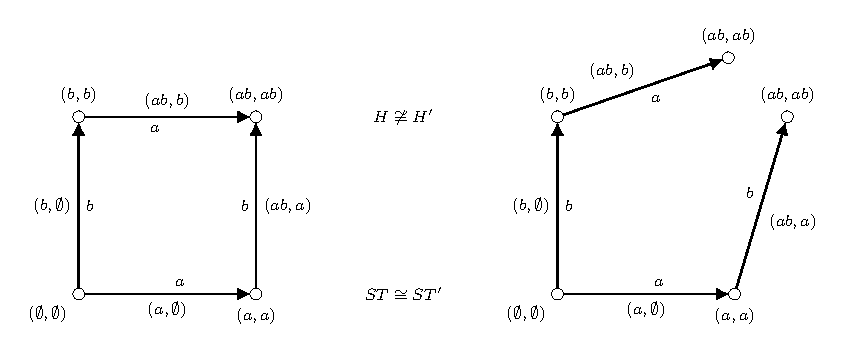
\includegraphics[scale=0.9]{Figures/4.Relationship-with-other-models-of-concurrency/ST-structure-and-HDA/HDA-collapse.pdf}
        \captionof{figure}[History unfolding of a square $\HDA$ through $\hintost$]{Example of ST-structures and higher-dimensional automata representing the unfoldings of a square $\HDA$ through $\hintost$. The ST-structure (left) is isomorphic to ST-structure (right). On the other hand, we see the higher-dimensional automaton (right) is not isomorphic to the higher-dimensional automaton (left). Since, the higher-dimensional automaton (right) has a split corner and the higher-dimensional automaton (left) is a nicely shaped square.}
        \label{fig:Unfolding-HDA}
    \end{figure}
    
    The mapping $\ST$ is not an embedding from $\allHDA$ to $\allST$ since it looses information, which in the example is the ability to announce the difference between when $a$ happens before $b$, or $b$ happens before $a$. This can also be seen, geometrically, as not being able to see the difference between the split corner of a square and a nicely shaped square.

    In Figure \ref{fig:asymmetric-conflict-st-hda}, we can see that higher-dimensional automata are not able to precisely identify events, but can be faithfully interpreted as ST-structures. ST-structures are able to precisely capture events while events in higher-dimensional automata are not easily captured. As we have shown in Figure \ref{fig:Unfolding-HDA}, ST-structures are not able to capture the difference between a higher-dimensional automaton and the unfolding of that higher-dimensional automaton. Hence, some processes might only be able to be represent as higher-dimensional automata, and identifying precisely these events of the processes would be challenging. We are interested in finding a model that is able to capture the aspect of higher-dimensional automata, but also be faithfully translated to ST-structures. In this regard, we will investigate Chu spaces and ST-structures.